%! TeX program = lualatex
\documentclass{article}

\usepackage[bezRozw]{../template} 
% \usepackage{../template} 

\title{Wielomiany}
\author{Weronika Jakimowicz}
\date{}

\begin{document}

\noindent\makebox[\linewidth]{\rule{\textwidth}{0.4pt}}

\textbf{\large Rozgrzewka}

\begin{zadanie}
  Ile jest dwucyfrowych liczb parzystych? Ile trzycyfrowych, a ile stucyfrowych?
\end{zadanie}

\begin{zadanie}
  Ile liczb  mniejszych od $1000$ jest podzielnych przez $3$ i $4$?
\end{zadanie}

\begin{zadanie}
  Ile jest przestawień (nie)słowa LEWINKLODZKI?
\end{zadanie}

\noindent\makebox[\linewidth]{\rule{\textwidth}{0.4pt}}

\begin{zadanie}
  A słowa MATEMATYKA?
\end{zadanie}

\begin{zadanie}
  Ile osób musiałoby urodzić się w Polsce jednego dnia, żeby zabrakło dla nich PESELi?
\end{zadanie}

\begin{zadanie}
  Ile jest przestawień liter $ABC$ i cyfr $1234$ tak, że najpierw stoją litery, a potem liczby? Ile jest przestawień, że litery nie stoją obok siebie?
\end{zadanie}

\begin{zadanie}
  W powiecie kłodzkim rejestracja samochodowa zaczyna się od $DKL$ i ma potem ciąg $5$ cyfr i liter, w którym wszystkie cyfry (których może być od $0$ do $5$) są zawsze przed literami. Ile jest możliwych rejestracji samochodów w powiecie kłodzkim?
\end{zadanie}

\begin{zadanie}
  Na ile sposobów można posadzić $150$ uczniów przy $150$-kątnym stole (lub okrągłym, jeśli takiego nie mamy pod ręką)?
\end{zadanie}

\begin{mybox}{Dwumian Newtona}
  Liczbę
  $$\binom{n}{k}=\frac{n!}{k!(n-k)!}$$
  nazywamy dwumianem Newtona. Warto kojarzyć tzw. \hl{trójkąt Pascala}
  \begin{center}
    \begin{tikzcd}[column sep=tiny, row sep=tiny]
      n=0 &   &   &   &   & 1 \\ 
      n=1 &   &   &   & 1 &   & 1 \\ 
      n=2 &   &   & 1 &   & 2 &   & 1\\ 
      n=3 &   & 1 &   & 3 &   & 3 &   & 1\\ 
      n=4 & 1 &   & 4 &   & 6 &   & 4 &   & 1
    \end{tikzcd}
  \end{center}
  \medskip
  który w wierszu $n$ ma wartości $\binom{n}{k}$ dla $k$ odpowiadającemu numerowi kolumny (licząc od $k=0$ do $k=n$).
\end{mybox}

\begin{zadanie}
  Chcemy się wszyscy na sali przywitać uściskiem dłoni. Ile zostanie wymienionych uścisków dłoni?
\end{zadanie}

\begin{zadanie}
  Chcemy wybrać $k$ osób spośród $30$. Na ile sposobów możemy to zrobić dla sensownych $k$?
\end{zadanie}

\begin{zadanie}
  W biegu niepodległości w Warszawie bierze udział $50$ biegaczy. Ile jest możliwych układów na podium?
\end{zadanie}

\begin{zadanie}
  Rzucamy $n$ rozróżnialnymi kośćmi. Na ile sposobów zobaczymy dokładnie $6$ jedynek i $3$ czwórki?
\end{zadanie}

\begin{zadanie}
  Zakładając, że jesteśmy po poniedziałku 4 XI 2024, zgadnij (warto spojrzeć na $\triangle$ Pascala) wzór na
  $$\sum_{k=0}^n\binom{n}{k}$$
  i udowodnij go indukcyjnie.
\end{zadanie}

\begin{zadanie}
  Robert budowniczy buduje ciągi składające się z $1$ i $2$, które sumują się do liczby $n$. Ile takich ciągów może ułożyć?
\end{zadanie}

\begin{zadanie}
  Mamy przejść szachownice $n\times k$ z jednego wierzchołka do przeciwnego poruszając się skokami po bokach pól. Ile jest możliwych dróg?
\end{zadanie}

\begin{zadanie}
  Ile wynosi $n$, jeśli liczba permutacji zbioru mającego $(n+1)$ elementów jest o $600$ większa od liczby permutacji zbioru mającego $n$ elementów?
\end{zadanie}

\begin{zadanie}
Do windy na ośmiopiętrowym budynku wsiadło $5$ osób. Na ile sposobów mogą opuścić na różnych piętrach windę?
\end{zadanie}

\begin{zadanie}
  Robert budowniczy buduje wieże wysokości $n$ z czerwonych i niebieskich bloków o wymiarach $1\times 1\times 1$. Ile różnych wież może ułożyć? 
\end{zadanie}
  
\begin{zadanie}
  Dodaj do siebie $n$ pierwszych liczb naturalnych. Teraz dodaj do siebie kwadraty $n$ pierwszych liczb naturalnych. 
\end{zadanie}

\begin{zadanie}
  Jeśli w poprzednim zadaniu nie korzystałeś do obliczania sumy kwadratów $\triangle$ Pascala, zrób to teraz. W przeciwnym przypadku pomyśl czy umiesz to zrobić bez $\triangle$ Pascala?
\end{zadanie}
\rozwiazanie{Chodzi o zapisani $\sum k^2=\sum [k(k+1)-k]$ suma $\sum k(k+1)$ to tak naprawdę $2\sum\binom{k+1}{2}$, a to wystarczy zejść o jedno w dół w trójkącie pascala, tzn. $\sum_1^n\binom{k+1}{2}=\binom{n+2}{3}$}

\begin{zadanie}
  Na ile sposobów można podzielić $2n$ elementowy zbiór na $n$ zbiorów $2$ elementowe? Co jeśli dzielimy $2n$ elementów na $n$ niepustych zbiorów? Czy umiesz policzyć na ile sposobów można podzielić zbiór o $(n+1)$ elementach na $k$ podzbiorów?
\end{zadanie}

\rozwiazanie{Liczby Stirlinga $\{n+1,k\}=k\{n,k\}+\{n,k-1\}$}

\rozwiazanie{Najpierw mamy kwadrat $n\times n$ bloczków, potem kładziemy na niego kwadrat $(n-1)\times (n-1)$ bloczków i tak dalej. Wynik to zliczenie rzędów z odpowiednią krotnością.
\begin{eqnarray}
\sum_{i=1}^{n}i^2&=&1\cdot(n+n-1)+2\cdot(n-1+n-2)+3\cdot(n-2+n-3)\\
&+&\cdots+(n-1)\cdot(2+1)+n\cdot1\\
&=&1\cdot(2n-1)+2\cdot(2n-3)+3\cdot(2n-5)+\cdots+(n-1)\cdot3+n\cdot1\\
&=&\sum_{i=1}^{n}i(2n-2i+1)\\
&=&2n\sum_{i=1}^{n}i-2\sum_{i=1}^{n}i^2+\sum_{i=1}^{n}i\\
\sum_{i=1}^{n}i^2&=&(2n+1)\sum_{i=1}^{n}i-2\sum_{i=1}^{n}i^2\\
3\sum_{i=1}^{n}i^2&=&(2n+1)\sum_{i=1}^{n}i\\
&=&\dfrac{n(n+1)(2n+1)}{2}\\
\sum_{i=1}^{n}i^2&=&\dfrac{n(n+1)(2n+1)}{6}
\end{eqnarray}
}

\def\n{\color{blue}N}
\def\c{\color{red}C}

\noindent\makebox[\linewidth]{\rule{\textwidth}{0.4pt}}

\textbf{\large Dla odważnych i o mocnym sercu}

\begin{zadanie}
  Na teren budowy na którym pracuje Robert przyszedł kierownik Józef i powiedział, że partia chce jak najczerwieńszą wieżę, więc co najwyżej dwa bloki niebieskie mogą stać jeden na drugim bez bycia rozdzielonym blokiem czerwonym. Tzn. wieże $\n\c\n\c\n\n\c$ i $\n\n\c\n\n$ są dozwolone, ale wieża $\c\c\c\c\c\n\c\c\c\n\n\c\c\c$ już nie. Co umiesz powiedzieć o ilości możliwych wież, które może wyprodukować Robert? 
\end{zadanie}

\begin{mybox}{Liczby modulo $\boldsymbol{p}$}
  Niech $p\in\N$ będzie liczbą pierwszą. Wtedy dowolna liczba $n\in\N$ zapisuje się jako $n=x\cdot p + y$, gdzie $y<p$ i $x\in\N$. Zbiór wszystkich możliwych $y$ (reszt z dzielenia przez $p$) oznaczamy $\Z_p$. Na $\Z_p$ mamy działanie $+_p$ dodawania modulo $p$, czyli gdy $a,b\in\Z_p$, to $a+_pb$ jest resztą z dzielenia $a+b$ przez $p$, np. $2+_53=0\in\Z_5$, $3+_53=1\in\Z_5$ czy $2+_73=5\in\Z_7$.
\end{mybox}

\begin{zadanie}
  Celem zadania będzie zliczenie prostych przechodzących przez $(0,0)$ na $\Z_p^2$, które dla $p=3$ wygląda następująco
  \begin{center}
    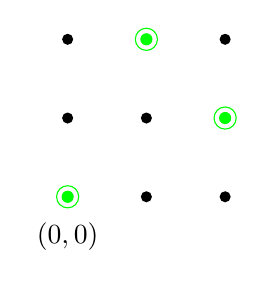
\begin{tikzpicture}
      \foreach \x in {0, 1, 2} {
        \foreach \y in {0, 1, 2} {
          \fill (\x, \y) circle (2pt);
        }
      }

      \fill[green](0, 0) circle (2.2pt);
      \fill[green](1, 2) circle (2.2pt);
      \fill[green](2, 1) circle (2.2pt);

      \draw[green](0,0) circle (4pt);
      \draw[green](1,2) circle (4pt);
      \draw[green](2,1) circle (4pt);

      \node at (0,-.5) {$(0,0)$};
      % \node at (1, -.5) {$(1, 0)$};
    \end{tikzpicture}
  \end{center}
  \begin{enumerate}
    \item Przykładowa prosta na $\Z_3^2$ została zaznaczona na rysunku wyżej. Narysuj kilka prostych na $\Z_p^2$ dla $p=2,3,5$.
    \item Ile punktów mają proste na $\R^2$? A ile na $\Z_p^3$?
    \item Wektor to strzałka narysowana na płaszczyźnie. Dowolny punkt połączony ze środkiem układu współrzędnych to wektor. To samo jest prawdziwe dla $\Z_p^2$. Czy umiesz powiedzieć ile jest niezerowych wektorów na $\Z_p^2$?
    \item Dla dowolnej prostej na płaszczyźnie możemy wybrać jej wektor kierunkowy, czyli strzałkę, która na niej leży (wskazuje kierunek w którym rośnie prosta). Rysunek niżej daje przykład kilku prostych na $\R^2$ i ich wektorów kierunkowych.
      \begin{center}
        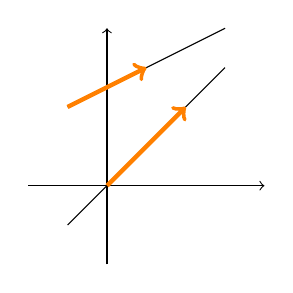
\begin{tikzpicture}
          \draw[->] (-1, 0)--(2, 0);
          \draw[->] (0, -1)--(0, 2);

          \draw (-.5,-.5)--(1.5,1.5);
          \draw[ultra thick, ->, orange] (0, 0)--(1, 1);

          \draw (-.5, 1)--(1.5, 2);
          \draw[ultra thick, ->, orange] (-.5, 1)--(.5,1.5);
        \end{tikzpicture}
      \end{center}
      Zauważmy, że wektor prosty jednoznacznie wyznacza prostą, ale prosta ma więcej niż jeden wektor kierunkowy (wystarczy przeskalować). To samo jest prawdziwe dla $\Z_p^2$.

      Korzystając z poprzednich podpunktów oblicz, ile jest prostych przechodzących przez zero na $\Z_p^2$.
  \end{enumerate}
  % Tak jak na $\R\times\R=\R^2$ umiemy rysować wektory i proste, tak analogicznie możemy to robić na kracie $\Z_p\times\Z_p$. Czy umiesz powiedzieć ile jest prostych na $\Z_p\times \Z_p$ dla $p=2,3,5$? A dla dowolnego $p$? A co jeśli chcemy liczyć proste w $\Z_p^3$?
\end{zadanie}

\noindent\makebox[\linewidth]{\rule{\textwidth}{0.4pt}}

\end{document}
